\section{Control Unit}

Στην παρούσα ενότητα υλοποιείται η μονάδα ελέγχου του σχήματος \ref{schematic:riscv} ως μηχανή πεπερασμένων καταστάσεων. Οι καταστάσεις της μηχανής είναι \texttt{IF} (instruction fetch), \texttt{ID} (instruction decoding), \texttt{EX} (execution), \texttt{MEM} (memory access) και \texttt{WB} (write back). Το διάγραμμα καταστάσεων φαίνεται στο διάγραμμα \ref{schematic:states}. Το διάγραμμα ροής του FSM φαίνεται στο σχήμα \ref{schematic:FSM}. Εφ' όσον η είσοδος επηρεάζει την έξοδο, το FSM είναι τύπου Mealy.\par

\begin{plotenv}[H]
	\centering
	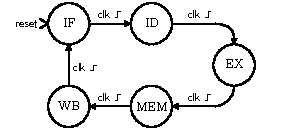
\includegraphics[height=2.2cm]{schematics/FSM_States.pdf}
	\caption{Διάγραμμα καταστάσεων. Το reset επαναφέρει τη μηχανή στην κατάσταση IF. Η μετάβαση στην επόμενη κατάσταση εκτελείται σε κάθε ανερχόμενη ακμή του ρολογιού.}
	\label{schematic:states}
\end{plotenv}

\begin{circuitfig}[H]
	\centering
	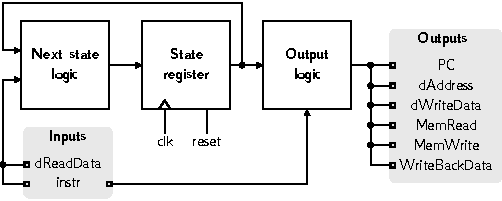
\includegraphics[width=8.4cm]{schematics/FSM.pdf}
	\caption{Διάγραμμα ροής του FSM.}
	\label{schematic:FSM}
\end{circuitfig}

Στο αρχείο \texttt{src/multicycle.v} δημιουργείται module με όνομα \texttt{multicycle} και εισόδους το ρολόι, σήμα reset, τα 32 bit της προς εκτέλεση εντολής και δεδομένα από την κύρια μνήμη. Οι έξοδοι του module είναι η διεύθυνση του PC, η διεύθυνση εγγραφής δεδομένων στην κύρια μνήμη, τα δεδομένα προς εγγραφή στην κύρια μνήμη,το σήμα ανάγνωσης από την κύρια μνήμη, το σήμα εγγραφής στην κύρια μνήμη και τα δεδομένα προς εγγραφή στο αρχείο καταχωρητών.\par
Οι παράμετροι που δηλώνονται εντός του module είναι τα \textsl{opcodes} και τα \textsl{funct3} πεδία των υποστηριζόμενων εντολών, και οι κωδικοί των πράξεων για την ALU όπως έχουν δηλωθεί και στο \texttt{src/alu.v}.\par
Αφότου γίνει instantiate του data path, ξεκινάει η περιγραφή της λογικής του FSM. Για τις πέντε καταστάσεις της μηχανής χρησιμοποιείται one-hot κωδικοποίηση.\par
Με ένα \texttt{always} block περιγράφεται η μνήμη των καταστάσεων. Το block εκτελείται στις ανερχόμενες ακμές του ρολογιού και έχει σύγχρονο reset το οποίο θέτει ως τρέχουσα κατάσταση την \texttt{IF}. Διαφορετικά, η τρέχουσα κατάσταση παίρνει την τιμή της επόμενης κατάστασης.\par
Ο προσδιορισμός της επόμενης κατάστασης γίνεται χρήσει ενός \texttt{always} block με την τρέχουσα κατάσταση στη λίστα ευαισθησίας. Η διαδοχή των καταστάσεων είναι $\texttt{IF}\to\texttt{ID}$, $\texttt{ID}\to\texttt{EX}$, $\texttt{EX}\to\texttt{MEM}$, $\texttt{MEM}\to\texttt{WB}$, $\texttt{WB}\to\texttt{IF}$. Η μετάβαση από τη μία κατάσταση στην επόμενη εξαρτάται μονάχα από την ταυτότητα της τρέχουσας κατάστασης.\par
Οι έξοδοι του FSM σε κάθε κατάσταση είναι ως εξής:
\begin{itemize}
	\item \texttt{IF}: τα σήματα RegWrite, MemToReg, PCSrc και loadPC μηδενίζονται.
	\item \texttt{ID}: στο στάδιο αυτό ρυθμίζεται το σήμα ALUCtrl βάσει του opcode της εντολής. \begin{itemize}
		      \item εάν το opcode της εντολής είναι STORE το ALUCtrl ρυθμίζεται στην πράξη της πρόσθεσης.
		      \item Εάν το opcode είναι LOAD, το ALUCtrl ρυθμίζεται και πάλι στην πράξη της πρόσθεσης.
		      \item εάν το opcode είναι BRANCH, το ALUCtrl ρυθμίζεται στην αφαίρεση. Δεν χρειάζεται να ελεγχθεί το πεδίο funct3 για opcode BRANCH καθότι στην προκειμένη υποστήριζεται μόνο η εντολή \texttt{BEQ}.
		      \item για opcode OP\_IMM το οποίο αντιστοιχεί στις εντολές τύπου I (πλην της \texttt{LW}) το ALUCtrl ρυθμίζεται βάση μόνον του funct3. Εξαίρεση αποτελούν οι εντολές ολίσθησης προς τα δεξιά. Το είδος της δεξιάς ολίσθησης, αριθμητική ή λογική, προσδιορίζεται από το bit 30. Ειδικότερα, εάν το bit 30 είναι μηδέν, η ολίσθηση είναι λογική. Διαφορετικά, εάν το bit 30 είναι μονάδα, η ολίσθηση είναι αριθμητική.
		      \item εάν το opcode είναι OP, το οποίο αντιστοιχεί στις εντολές τύπου R, η ρύθμιση του ALUCtrl εξαρτάται από το funct7 και το funct3. Εάν το funct7 είναι $(0000000)_\mathrm{BIN}$, το ALUCtrl ρυθμίζεται απευθείας βάση του funct3. Εάν το funct7 είναι  $(01000000)_\mathrm{BIN}$ και το πεδίο funct3 είναι $(000)_\mathrm{BIN}$ τότε η πράξη της ALU θα είναι αφαίρεση. Εάν το funct3 είναι $(101)_\mathrm{BIN}$ η πράξη της ALU θα είναι αριθμητική ολίσθηση προς τα δεξιά. Ο διαχωρισμός ως προς το funct7 είναι απαραίτητος διότι οι εντολές \texttt{SUB} και \texttt{ADD} έχουν το ίδιο funct7. Ομοίως και οι εντολές \texttt{SRA} και \texttt{SRL} έχουν το ίδιο funct7.
	      \end{itemize} Επιπλέον, ρυθμίζεται το σήμα επιλογής του δεύτερου τελεσταίου της ALU. Για εντολές με opcode LOAD, STORE ή OP\_IMM το ALUSrc παίρνει την τιμή $1$ και ο δεύτερος τελεσταίος της ALU θα είναι ο immediate πλάτους 32 bit. Για όλα τα υπόλοιπα opcodes το ALUSrc απενεργοποιείται και ο δεύτερος τελεσταίος είναι τα δεδομένα του της δεύτερης διεύθυνσης που δίνεται ως είσοδος στο αρχείο καταχωρητών.
	\item \texttt{EX}: δεν τροποποιούνται οι έξοδοι του FSM σε αυτό το στάδιο.
	\item \texttt{MEM}: τα σχετικά με την κύρια μνήμη σήματα ρυθμίζονται βάσει του opcode της εντολής. \begin{itemize}
		      \item LOAD: το σήμα ανάγνωσης από τη μνήμη ενεργοποιείται και το σήμα εγγραφής στην μνήμη απενεργοποιείται.
		      \item STORE: το σήμα ανάγνωσης από τη μνήμη απενεργοποιείται και ενεργοποιείται το σήμα εγγραφής στη μνήμη.
		      \item BRANCH: απενεργοποιούνται τα σήματα εγγραφής και ανάγνωσης από τη μνήμη. Επιπλέον, ρυθμίζεται το σήμα PCSrc το οποίο ελέγχει την επόμενη τιμή του PC. Εάν το αποτέλεσμα της ALU είναι μηδέν, τότε ακολουθείται το branch και το PCSrc σήμα γίνεται $1$. Διαφορετικά, το σήμα PCSrc γίνεται $0$.
		    \item Η προκαθορισμένη συμπεριφορά είναι τα σήματα ανάγνωσης και εγγραφής στη μνήμη να είναι απενεργοποιημένα.
	      \end{itemize}
	\item \texttt{WB}: σε αυτό το στάδιο ενεργοποιείται το σήμα loadPC για την φόρτωση της επόμενης εντολής, απενεργοποιούνται τά σήματα ανάγνωσης και εγγραφής στην κύρια μνήμα και ρυθμίζονται τα σήματα εγγραφής στο αρχείο καταχωρητών βάση των opcodes.\begin{itemize}
		      \item LOAD: το σήμα εγγραφής στο αρχείο καταχωρητών και το σήμα εγγραφής δεδομένων που προέρχονται από τη μνήμη ενεργοποιούνται.
		      \item STORE: το σήμα εγγραφής στο αρχείο καταχωρητών και το σήμα εγγραφής δεδομένων που προέρχονται από τη μνήμη απενεργοποιούνται.
		      \item Λοιπά opcodes: το σήμα εγγραφής στο αρχείο καταχωρητών ενεργοποιείται και το σήμα εγγραφής δεδομένων που προέρχονται από τη μνήμη απενεργοποιείται.
	      \end{itemize}
\end{itemize}

\subsection{Testbench}

Στο αρχείο \texttt{src/top\_proc\_TB.v} γίνεται instantiate του module της μνήμης εντολών, του module της μνήμης δεδομένων και του module του control unit. Σε ένα \texttt{initial} block ενεργοποιείται το ρολόι και το σήμα reset το οποίο μένει ενεργό και $30\unit{\nano\second}$. Εντός ενός \texttt{always} block ανά $10\unit{\nano\second}$ συμπληρώνεται το σήμα του ρολογιού. Επομένως, η περίοδος του ρολογιού είναι $T=20\unit{\nano\second}$. Τέλος, η προσομοίωση ολοκληρώνεται μετά από $100\unit{\micro\second}$.\par

Το αρχείο \texttt{sc/rom\_bytes.data} περιέχει τα δεδομένα της μνήμης εντολών. Προκειμένου να γίνει πιο εύκολος ο έλεγχος του χρονοδιαγράμματος οι εντολές, μέσω ενός python script (\texttt{util/instructions.py}) που συνοδεύει την παρούσα αναφορά, αποκωδικοποιήθηκαν σε γλώσσα assembly και δίνονται στο listing \ref{lst:instructions}. Τα immediates έχουν αποκωδικοποιηθεί σε προσημανσμένη δεκαδική μορφή.\par

\lstdefinelanguage{Assembler}{
	morekeywords={
			addi, andi, ori, xori, slti, sltiu, slli, srli, srai, lui, auipc, add, sub, sll, slt, sltu, xor, srl, sra, or, and, beq, bne, blt, bge, bltu, bgeu, jal, jalr, lw, lh, lhu, lb, lbu, sw, sh, sb, lui, auipc, fence, fence.i, ecall, ebreak, csrrw, csrrs, csrrc, csrrwi, csrrsi, csrrci, mret, sret, uret, wfi, sfence.vma
		},
	sensitive=true,
	morecomment=[l]{\#},
	commentstyle=\ttfamily,
	morestring=[b]",
}

\begin{lstlisting}[language=Assembler,tabsize=4,basicstyle=\ttfamily,caption={Περιεχόμενα μνήμης εντολών σε μορφή γλώσσας assembly. Τα πεδία των καταχωρητών εμφανίζονται με τη σειρά του σχήματος \ref{schematic:instructions}},label={lst:instructions}]
addi x1, x0, 4		#0x0000
addi x2, x0, 1		#0x0004
addi x3, x0, 3		#0x0008
addi x4, x0, 7		#0x000C
addi x5, x0, -2		#0x0010
add x6, x3, x3		#0x0014
sub x7, x6, x5		#0x0018
sll x8, x3, x2		#0x001C
slt x9, x8, x4		#0x0020
xor x10, x1, x7		#0x0024
srl x11, x10, x9	#0x0028
and x12, x3, x6		#0x002C
or x13, x10, x12	#0x0030
sra x14, x5, x2		#0x0034
sw x10, 0(x2)		#0x0038
lw x15, 0(x2)		#0x003C
andi x16, x13, 7	#0x0040
ori x17, x13, 4		#0x0044
srli x18, x4, 3		#0x0048
beq x6, x8, 6		#0x004C
None				#0x0050
None				#0x0054
None				#0x0058
None				#0x005C
None				#0x0060
None				#0x0064
None				#0x0068
None				#0x006C
None				#0x0070
None				#0x0074
None				#0x0078
xori x19, x11, 12	#0x007C
slli x20, x19, 1	#0x0080
srai x21, x5, 1026	#0x0084
slti x22, x20, 28	#0x0088
None				#0x008C
\end{lstlisting}

Στο χρονοδιάγραμμα \ref{waveform:tb5} τα σήματα immediate\_32, op1, op2 και result εκτυπώνονται με προσημανσμένη μορφή στο δεκαδικό σύστημα. Το σήμα του ρολογιού εκτυπώνεται πολλές φορές για ευκολία ανάγνωσης των κυματομορφών.\par

\begin{plotenv}[H]
	\centering
	\includegraphics[width=\linewidth]{waveforms/tb5_1.png}
% \end{plotenv}
% \begin{plotenv}[H]
	\centering
	\includegraphics[width=\linewidth]{waveforms/tb5_2.png}
% \end{plotenv}
% \begin{plotenv}[H]
	\centering
	\includegraphics[width=\linewidth]{waveforms/tb5_3.png}
% \end{plotenv}
% \begin{plotenv}[H]
	\centering
	\includegraphics[width=\linewidth]{waveforms/tb5_4.png}
	\caption{Χρονοδιάγραμμα για τον επεξεργαστή του σχήματος \ref{schematic:riscv}.}
	\label{waveform:tb5}
\end{plotenv}

Στο \textbf{πρώτο εκ των τεσσάρων διαγραμμάτων}, η πρώτη εντολή αποθηκεύει την τιμή $4$ στον καταχωρητή \texttt{x1} προσθέτοντας το $4$ στο περιεχόμενο του \texttt{x0} το οποίο είναι μηδέν. Ο πρώτος τελεσταίος είναι $0$ και ο δεύτερος έχει την τιμή του immediate, $4$. Το αποτέλεσμα είναι $4$ και το wrideData είναι επίσης $4$. Οι επόμενες τέσσερις εντολές ακολουθούν την ίδια λογική. Η δεύτερη, κατά σειρά εκτέλεσης, εντολή γράφει την τιμή $1$ στον καταχωρητή \texttt{x2}. Το op1 είναι $0$, το op2 είναι $1$, το result είναι $1$ και το writeData είναι επίσης $1$. Η τρίτη, κατά σειρά εκτέλεσης, εντολή γράφει την τιμή $3$ στον καταχωρητή \texttt{x3}. Το op1 είναι $0$, το op2 είναι $3$, το result είναι $1$ και το writeData είναι επίσης $3$. Η τέταρτη, κατά σειρά εκτέλεσης, εντολή γράφει την τιμή $7$ στον καταχωρητή \texttt{x4}. Το op1 είναι $0$, το op2 είναι $7$, το result είναι $1$ και το writeData είναι επίσης $7$. Η πέμπτη, κατά σειρά εκτέλεσης, εντολή γράφει την τιμή $-2$ στον καταχωρητή \texttt{x5}. Το op1 είναι $0$, το op2 είναι $-2$, το result είναι $-2$ και το writeData είναι επίσης $(-2)_\mathrm{DEC}=(4294967294)_\mathrm{HEX}$.
Η έκτη εντολή προσθέτει το περιεχόμενο του καταχωρήτη \texttt{x3} στο περιοχόμενο του καταχωρητή \texttt{x3} και αποθηκεύει το αποτέλεσμα στον καταχωρητή \texttt{x6}. Όντως, τα rs1 και rs2 έχουν την τιμή $03$, τα op1 και op2 έχουν τιμή $3$, το rd έχει την τιμή $6$ και το result και το writeData έχουν την τιμή $6$. Στην επόμενη εντολή, από το περιεχόμενο του καταχωρητή \texttt{x6} αφαιρείται το περιοχόμενο του \texttt{x5} και το αποτέλεσμα αποθηκεύεται στον καταχωρητή \texttt{x7}. Πράγματι, το rs1 είναι 6, το rs2 είναι 5 και το rd είναι 7. Το αποτέλεσμα είναι $8$ και το writeData είναι επίσης $8$, αφού op1 είναι $6$ και op2 είναι $-2$. Στην επόμενη εντολή, το περιεχόμενο του καταχωρητή \texttt{x3} ολισθαίνει κατά 1 bit προς τα αριστερά και το αποτέλεσμα αποθηκεύεται στον καταχωρητή \texttt{x8}. Το rs1 είναι $3$, το rs2 είναι $2$ και το rd είναι $8$. Το op1 είναι $3$ και το op2 είναι $1$. Το αποτέλεσμα είναι $6$, αφού η ολίσθηση αριστερά κατά 1 bit ισοδυναμεί με διπλασιασμό της τιμής και το writeData είναι επίσης $6$. Στην επόμενη εντολή, το περιεχόμενο του καταχωρητή \texttt{x8} συγκρίνεται με το περιεχόμενο του καταχωρητή \texttt{x4}. Επειδή το \texttt{x8} είναι μικρότερο του \texttt{x4}, το αποτέλεσμα της σύγκρισης είναι $1$ και το writeData είναι επίσης $1$ το οποίο σύμφωνα με την εντολή αποθηκεύεται στον \texttt{x7} και επιβεβαιώνεται αφού rd είναι 7. Στην δέκατη εντολή, το αποτέλεσμα της αποκλειστικής διάζευξης μεταξύ των bit των \texttt{x1} και \texttt{x7} αποθηκεύεται στον καταχωρητή \texttt{x10}. Το op1 είναι $4=(0100)_\mathrm{BIN}$ και το op2 είναι $8=(1000)_\mathrm{BIN}$. Το result είναι $12=(1100)_\mathrm{BIN}$ και το rd είναι $10=(0Α)_\mathrm{ΗΕΧ}$.\par
Στο \textbf{δεύτερο εκ των τεσσάρων διαγραμμάτων} η πρώτη εντολή που εκτελείται (PC$=(00400028)_\mathrm{HEX}$) είναι δεξιά ολίσθηση του \texttt{x10} \texttt{x10}$[4:0]$, δηλαδή κατά 1 bit. Το αποτέλεσμα είναι $6$, αφού η δεξιά ολίσθηση κατά 1 bit ισοδυναμεί με υποδιπλασιασμό και το writeData είναι επίσης $6$. Στην επόμενη εντολή πραγματοποιείται λογική σύζευξη των περιοχομένων των \texttt{x3} και \texttt{x6} και το αποτέλεσμα αποθηκέυεται στον \texttt{x12}. Είναι op1$=6=(110)_\mathrm{BIN}$ και op2$=6=(011)_\mathrm{BIN}$. Το result σήμα έχει την τιμή $2=(010)_\mathrm{BIN}$ και είναι σωστή. Στην επόμενη εντολή, εκτελείται λογική διάζευξη των περιεχομένων των \texttt{x10} και \texttt{x12}. To op1 είναι $12=(1100)_\mathrm{BIN}$ και το op2 είναι $2=(0010)_\mathrm{BIN}$ (εξαιτίας της προηγούμενης εντολής). Το αποτέλεσμα θα πρέπει να είναι $14=(1110)_\mathrm{BIN}$ το οποίο επιβεβαιώνεται από το χρονοδιάγραμμα. Αμέσως μετά, το περιεχόμενο το \texttt{x5} υφίσταται αριθμητική ολίσθηση προς τα δεξιά κατά \texttt{x2}$[4:0]$ και το αποτέλεσμα αποθηκεύεται στον \texttt{x14}. Το op1 είναι $-2=(1\ldots10)_\mathrm{BIN,signed}$ και το op2 $1$. Το αποτέλεσμα θα πρέπει να είναι $-1$ και πράγματι ισχύει.\par
Έπειτα, δοκιμάζονται οι εντολές προσπέλασης της μνήμης. Για PC$=(00400038)_\mathrm{HEX}$ αποθηκεύεται στη μνήμη στη διεύθυνση που δείχνει ο καταχωρητής \texttt{x2} η τιμή του καταχωρητή \texttt{x10}. Το σήμα MemWrite γίνεται ενεργό για έναν κύκλο και η τιμή που γράφεται στη μνήμη θα πρέπει να είναι $12$. Όντως, τo dWriteData είναι $12=(0C)_\mathrm{HEX}$. Αμέσως μετά, η τιμή που γράφθηκε στη μνήμη διαβάζεται και αποθηκεύται στον καταχωρητή \texttt{x15}. Tα σήματα MemToReg και MemRead ενεργοποιούνται το καθένα για ένα κύκλο και συγκεκριμένα, το MemRead ενεργοποιείται στον κύκλο πριν το MemToReg. Η τιμή που γράφεται στο αρχείο καταχωρητών είναι WriteData$=12$ όπως ήταν και το αναμενόμενο.\par
Η επόμενη εντολή εκτελεί λογική σύζευξη των bit του καταχωρητή \texttt{x13} με την τιμή $7=(00111)_\mathrm{BIN}$ και το αποτέλεσμα αποθηκεύεται στον καταχωρητή \texttt{x16}. Η τιμή του \texttt{x13} (op1) είναι $14=(01110)_\mathrm{BIN}$. Το WriteData έχει την σωστή τιμή $6=(00110)_\mathrm{BIN}$. Η επόμενη εντολή εκτελεί λογική διάζευξη των bit του καταχωρητή \texttt{x13} με την τιμή $4=(00100)_\mathrm{BIN}$ και το αποτέλεσμα αποθηκεύεται στον καταχωρητή \texttt{x17}. Η τιμή του \texttt{x13} (op1) είναι $14=(01110)_\mathrm{BIN}$. Το WriteData έχει την σωστή τιμή $14=(01110)_\mathrm{BIN}$. Αμέσως μετά, εκτελείται δεξιά λογική ολίσθηση κατά 3 στον καταχωρητή \texttt{x4} και το αποτέλεσμα αποθηκεύεται στον \texttt{x18}. Είναι op1$=7=(0111)_\mathrm{BIN}$ και op2$=3$. Το αποτέλεσμα είναι σωστά $0$ και ενεργοποιείται το σήμα Zero της ALU. Τελευταία εντολή στο δεύτερο διάγραμμα είναι branch on equal. Συγκρίνεται η τιμή του \texttt{x6} με την τιμή του \texttt{x8}. Επειδή είναι ίσες, το αποτέλεσμα της σύγκρισης είναι $1$ και το Zero σήμα παραμένει ενεργό. Άρα το νέο PC θα υπολογιστεί με βάση το branch offset.\par
Στο \textbf{τρίτο εκ των τεσσάρων διαγραμμάτων} η πρώτη εντολή που εκτελείται είναι η εντολή στη διέυθυνση $(0040050)_\mathrm{HEX}$ αφού η προηγούμενη εντολή ήταν branch και το Zero της ALU ήταν ενεργό. Η εντολή στην τρέχουσα διεύθυνση δεν εκτελεί κάποια πράξη. Δεν ισοδυναμεί αυστηρά με την \texttt{NOP} στο επίπεδο της κωδικοποίησης αλλά το αποτέλεσμα είναι ακριβώς το ίδιο. Η επόμενη όχι \texttt{NOP} εντολή εκτελείται στη διεύθυνση $(004007C)_\mathrm{HEX}$. Επόμενη εντολή είναι αποκλειστική διάζευξη με immediate. Τα op1 και op2 είναι σωστά και το αποτέλεσμα είναι $10=(01010)_\mathrm{BIN}$. Η επόμενη εντολή, ολισθαίνει αριστερά το περιοχόμενο του \texttt{x19} κατά 1 bit. Το αποτέλεσμα θα πρέπει να είναι το διπλάσιο της προηγούμενης τιμής του \texttt{x19} το οποίο επιβεβαιώνεται. Η προτελευταία εντολή είναι αριθμητική ολίσθηση προς τα δεξιά του καταχωρήτή \texttt{x5} (op1$=-2=(1\ldots10)_\mathrm{BIN}$) κατά 2. Το αποτέλσμα θα είναι $(1\ldots 1)_\mathrm{BIN}=-1$. Απομένει μία εντολή σύγκρισης με immediate. Γίνεται η σύγκριση $28<\texttt{x20}$. Από την παραπροηγούμενη εντολή η τιμή του \texttt{x20} είναι $20$. Άρα το αποτέλεσμα είναι μηδέν.\par

Η ορθή λειτουργία του επεξεργαστή έχει επαληθευθεί βάσει των αποτελεσμάτων του χρονοδιαγράμματος \ref{waveform:tb5}.\par